% Options for packages loaded elsewhere
\PassOptionsToPackage{unicode}{hyperref}
\PassOptionsToPackage{hyphens}{url}
%
\documentclass[
]{article}
\usepackage{lmodern}
\usepackage{amssymb,amsmath}
\usepackage{ifxetex,ifluatex}
\ifnum 0\ifxetex 1\fi\ifluatex 1\fi=0 % if pdftex
  \usepackage[T1]{fontenc}
  \usepackage[utf8]{inputenc}
  \usepackage{textcomp} % provide euro and other symbols
\else % if luatex or xetex
  \usepackage{unicode-math}
  \defaultfontfeatures{Scale=MatchLowercase}
  \defaultfontfeatures[\rmfamily]{Ligatures=TeX,Scale=1}
\fi
% Use upquote if available, for straight quotes in verbatim environments
\IfFileExists{upquote.sty}{\usepackage{upquote}}{}
\IfFileExists{microtype.sty}{% use microtype if available
  \usepackage[]{microtype}
  \UseMicrotypeSet[protrusion]{basicmath} % disable protrusion for tt fonts
}{}
\makeatletter
\@ifundefined{KOMAClassName}{% if non-KOMA class
  \IfFileExists{parskip.sty}{%
    \usepackage{parskip}
  }{% else
    \setlength{\parindent}{0pt}
    \setlength{\parskip}{6pt plus 2pt minus 1pt}}
}{% if KOMA class
  \KOMAoptions{parskip=half}}
\makeatother
\usepackage{xcolor}
\IfFileExists{xurl.sty}{\usepackage{xurl}}{} % add URL line breaks if available
\IfFileExists{bookmark.sty}{\usepackage{bookmark}}{\usepackage{hyperref}}
\hypersetup{
  pdftitle={How to calibrate protection vulnerability scoring?},
  pdfauthor={Field experience stocktaking - UNHCR},
  hidelinks,
  pdfcreator={LaTeX via pandoc}}
\urlstyle{same} % disable monospaced font for URLs
\usepackage[margin=1in]{geometry}
\usepackage{longtable,booktabs}
% Correct order of tables after \paragraph or \subparagraph
\usepackage{etoolbox}
\makeatletter
\patchcmd\longtable{\par}{\if@noskipsec\mbox{}\fi\par}{}{}
\makeatother
% Allow footnotes in longtable head/foot
\IfFileExists{footnotehyper.sty}{\usepackage{footnotehyper}}{\usepackage{footnote}}
\makesavenoteenv{longtable}
\usepackage{graphicx,grffile}
\makeatletter
\def\maxwidth{\ifdim\Gin@nat@width>\linewidth\linewidth\else\Gin@nat@width\fi}
\def\maxheight{\ifdim\Gin@nat@height>\textheight\textheight\else\Gin@nat@height\fi}
\makeatother
% Scale images if necessary, so that they will not overflow the page
% margins by default, and it is still possible to overwrite the defaults
% using explicit options in \includegraphics[width, height, ...]{}
\setkeys{Gin}{width=\maxwidth,height=\maxheight,keepaspectratio}
% Set default figure placement to htbp
\makeatletter
\def\fps@figure{htbp}
\makeatother
\setlength{\emergencystretch}{3em} % prevent overfull lines
\providecommand{\tightlist}{%
  \setlength{\itemsep}{0pt}\setlength{\parskip}{0pt}}
\setcounter{secnumdepth}{5}
\usepackage{booktabs}
\usepackage{amsthm}
\makeatletter
\def\thm@space@setup{%
  \thm@preskip=8pt plus 2pt minus 4pt
  \thm@postskip=\thm@preskip
}
\makeatother
\usepackage[]{natbib}
\bibliographystyle{apalike}

\title{How to calibrate protection vulnerability scoring?}
\author{Field experience stocktaking - UNHCR}
\date{V0.1 - Draft Version for peer review - as of 01 March 2021}

\begin{document}
\maketitle

{
\setcounter{tocdepth}{2}
\tableofcontents
}
\hypertarget{introduction}{%
\section{Introduction}\label{introduction}}

Official UNHCR guidance on how to measure vulnerability are the following:

\begin{quote}
UNHCR measures indicators of refugee well-being including health and nutrition status, water and sanitation, shel-ter, socio- economic poverty and protection vulnerabilities to guide assistance and solution strategies. Analysis of individual protection vulnerabilities is guided by the Specific Needs approach, which guides case management. UN-HCR Specific Needs codes are outlined in Annex 2. In addition UNHCR promotes the inclusion of refugees into Na-tional Poverty Assessments so as to be able to generate comparable data between refugees and host communities. Comparable socio-economic data is increasingly important to ascertain the level of assistance needed and to inform regional area-based development programs implemented by development and private sector partners together with National Governments as part of the Global Compact for Refugees
-- \href{https://www.unhcr.org/5ef9ba0d4.pdf\#page=11}{UNHCR/WFP Joint Guidance: Targeting of Assistance to Meet Basic Needs}
\end{quote}

This is complemented by the guidance below:

\begin{quote}
\textbf{Vulnerability analysis framework}: The framework defines which households are vulnerable among the entire refugee population. Various socio-economic or sector models can be applied as tools to prioritize who is eligible to receive assistance. An efficient tool for predicting the welfare of all refugee households is econometric welfare modelling. An example can be found in the Vulnerability Assessment Framework in Jordan
\end{quote}

\begin{quote}
\textbf{Targeting: defining eligibility}: Anchored in a rights-based approach, the identification and selection of individuals or households for appropriate assistance are based on multi-sectoral analysis of protection risks, wealth and food insecurity, the vulnerability framework and the identified needs. Information from monitoring is analysed and can be used to update targeting eligibility criteria and make other adjustments.
-- \href{https://www.unhcr.org/590aefc77}{Basic Needs Approach in the Refugee Response}
\end{quote}

WFP has quite detailed guidance around a \href{https://resources.vam.wfp.org/data-analysis/quantitative/food-security/cari-the-consolidated-approach-for-reporting-indicators-of-food-security}{Consolidated Approach for reporting indicators of food security, (CARI)} which allow to define a composite indicator the ``Food Security Index''

\begin{figure}
\centering
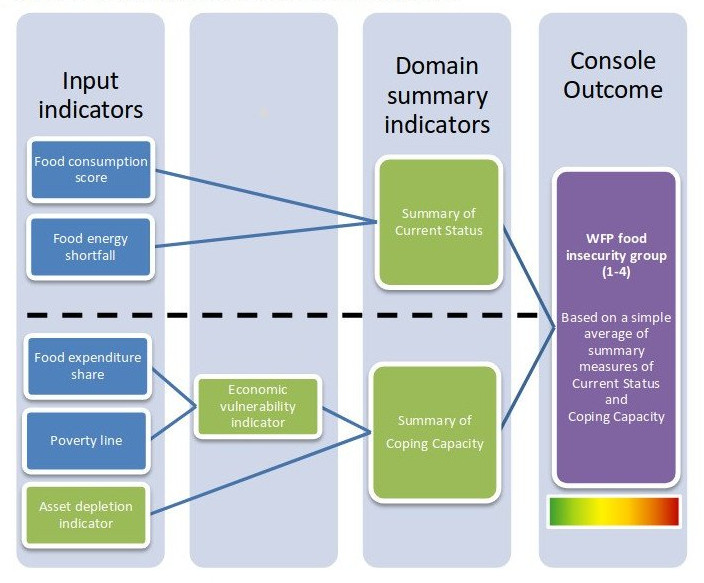
\includegraphics{media/cari.jpg}
\caption{CARI Food Security Index theoretical model}
\end{figure}

UNHCR Existing Guidance not provide details on how the calculation shall be made. This document build on \href{https://composite-indicators.jrc.ec.europa.eu/?q=10-step-guide}{generic guidance on composite indicator development from the EU-joint Research Center on Composite Indicator} and aims at providing a cookbook approach for field practitionners. This document is build with a reproducible analysis approach, which implies for data expert on the field can simply adapt the scripts included in the documents to the context and data available in their own operations.

\hypertarget{executive-summary-what-you-need-to-know-as-a-manager}{%
\section{Executive summary: what you need to know as a manager}\label{executive-summary-what-you-need-to-know-as-a-manager}}

\hypertarget{theres-no-simple-solution-to-complex-problem}{%
\subsection{There's no simple solution to complex problem}\label{theres-no-simple-solution-to-complex-problem}}

\hypertarget{scoring-with-a-protection-lens}{%
\subsection{Scoring with a protection lens}\label{scoring-with-a-protection-lens}}

\hypertarget{be-ready-for-auditing}{%
\subsection{Be ready for auditing}\label{be-ready-for-auditing}}

\hypertarget{why-and-when-using-vulnerability-scoring}{%
\section{Why and when using vulnerability scoring?}\label{why-and-when-using-vulnerability-scoring}}

\hypertarget{from-the-identification-of-vulnerables-to-the-scoring-of-household-vulnerability}{%
\subsection{from the identification of vulnerables to the scoring of household vulnerability}\label{from-the-identification-of-vulnerables-to-the-scoring-of-household-vulnerability}}

\hypertarget{different-models-of-vulnerability-food-insecurity-poverty-protection}{%
\subsection{Different models of vulnerability: food insecurity, poverty, protection}\label{different-models-of-vulnerability-food-insecurity-poverty-protection}}

\hypertarget{potential-approaches-to-calibrate-scores}{%
\section{Potential approaches to calibrate scores}\label{potential-approaches-to-calibrate-scores}}

\hypertarget{what-is-calibration}{%
\subsection{What is calibration?}\label{what-is-calibration}}

\hypertarget{calibration-using-expert-opinions}{%
\subsection{Calibration using expert opinions}\label{calibration-using-expert-opinions}}

\hypertarget{calibration-using-statistically-representative-dataset}{%
\subsection{Calibration using statistically representative dataset}\label{calibration-using-statistically-representative-dataset}}

\hypertarget{risks-when-calibrating-vulnerability-scores}{%
\section{Risks when calibrating vulnerability scores}\label{risks-when-calibrating-vulnerability-scores}}

\hypertarget{theres-no-magic-formula}{%
\subsection{There's no magic formula}\label{theres-no-magic-formula}}

\hypertarget{building-consensus}{%
\subsection{Building consensus}\label{building-consensus}}

\hypertarget{including-and-communication-with-communities}{%
\subsection{Including and communication with communities}\label{including-and-communication-with-communities}}

\hypertarget{budget-allocation}{%
\section{Budget allocation}\label{budget-allocation}}

\hypertarget{selecting-experts}{%
\subsection{Selecting experts}\label{selecting-experts}}

\hypertarget{speed-up-consultation-with-quadratic-voting}{%
\subsection{Speed-up consultation with quadratic voting}\label{speed-up-consultation-with-quadratic-voting}}

\hypertarget{restitution-of-results}{%
\subsection{Restitution of results}\label{restitution-of-results}}

\hypertarget{conjoint-analysis}{%
\section{Conjoint analysis}\label{conjoint-analysis}}

\hypertarget{principle-of-opinion-reverse-engineering}{%
\subsection{Principle of opinion reverse engineering}\label{principle-of-opinion-reverse-engineering}}

\hypertarget{cutomise-the-indicators}{%
\subsection{Cutomise the indicators}\label{cutomise-the-indicators}}

\hypertarget{setting-up-the-consultation}{%
\subsection{Setting up the consultation}\label{setting-up-the-consultation}}

\hypertarget{analytic-hierarchy-process}{%
\section{Analytic Hierarchy Process}\label{analytic-hierarchy-process}}

\hypertarget{section}{%
\subsection{}\label{section}}

\hypertarget{vulnerability-proxy-regression}{%
\section{Vulnerability proxy Regression}\label{vulnerability-proxy-regression}}

\hypertarget{section-1}{%
\subsection{}\label{section-1}}

\hypertarget{data-envelopment-and-deprivation}{%
\section{Data Envelopment and Deprivation}\label{data-envelopment-and-deprivation}}

\hypertarget{what-is-deprivation-analysis}{%
\subsection{What is deprivation analysis?}\label{what-is-deprivation-analysis}}

\hypertarget{robustness-and-sensitivity-analysis}{%
\section{Robustness and Sensitivity analysis}\label{robustness-and-sensitivity-analysis}}

\hypertarget{section-2}{%
\subsection{}\label{section-2}}

\hypertarget{item-response-theory}{%
\section{Item Response Theory}\label{item-response-theory}}

\hypertarget{section-3}{%
\subsection{}\label{section-3}}

\hypertarget{eligibility-and-prioritization}{%
\section{Eligibility and Prioritization}\label{eligibility-and-prioritization}}

\hypertarget{eligibility}{%
\subsection{Eligibility}\label{eligibility}}

\hypertarget{conclusion}{%
\section{Conclusion}\label{conclusion}}

\hypertarget{section-4}{%
\subsection{}\label{section-4}}

  \bibliography{refs.bib}

\end{document}
